\let\negmedspace\undefined
\let\negthickspace\undefined
\documentclass[journal,12pt,onecolumn]{IEEEtran}
\usepackage{cite}
\usepackage{amsmath,amssymb,amsfonts,amsthm}
\usepackage{algorithmic}
\usepackage{graphicx}
\usepackage{textcomp}
\usepackage{xcolor}
\usepackage{txfonts}
\usepackage{listings}
\usepackage{enumitem}
\usepackage{mathtools}
\usepackage{gensymb}
\usepackage{comment}
\usepackage{caption}
\usepackage[breaklinks=true]{hyperref}
\usepackage{tkz-euclide} 
\usepackage{listings}
\usepackage{gvv}                                        
%\def\inputGnumericTable{}                                 
\usepackage[latin1]{inputenc}     
\usepackage{xparse}
\usepackage{color}                                            
\usepackage{array}                                            
\usepackage{longtable}                                       
\usepackage{calc}                                             
\usepackage{multirow}
\usepackage{multicol}
\usepackage{hhline}                                           
\usepackage{ifthen}                                           
\usepackage{lscape}
\usepackage{tabularx}
\usepackage{array}
\usepackage{float}
%\newtheorem{theorem}{Theorem}[section]
%\newtheorem{theorem}{Theorem}[section]
%\newtheorem{problem}{Problem}
%\newtheorem{proposition}{Proposition}[section]
%\newtheorem{lemma}{Lemma}[section]
%\newtheorem{corollary}[theorem]{Corollary}
%\newtheorem{example}{Example}[section]
%\newtheorem{definition}[problem]{Definition}

\begin{document}

\title{1.8.11}
\author{AI25BTECH11035 - SUJAL RAJANI}
% \maketitle
% \newpage
% \bigskip
%\begin{document}
{\let\newpage\relax\maketitle}
%\renewcommand{\thefigure}{\theenumi}
%\renewcommand{\thetable}{\theenumi}
% \newpage
% \bigskip
\textbf{Question}:
\\
\noindent Find the coordinates of the point $\vec{P}$ on AD such that AP : PD = 2 : 1. 
\\
\textbf{Solution:} 
\\
As nothing is mentioned in the question about the coordinates of A and D , so we are assuming the coordinates of A as (2,2) ,D as (-1,-1) .
\begin{align}
			\vec A = \myvec{2\\2},\vec D = \myvec{-1\\-1}.
\end{align}
as mentioned in the question $\vec{P}$ is dividing the join of A and D in $2:1$.

so for finding the position vector of $\vec{P}$ we are using section formula 
\\
If $\vec{D}$ divides BC in the ratio k : 1
\begin{align*}
     \vec{D}=\dfrac{k\vec{C}+\vec{B}}{k+1}
\end{align*}
\\
\quad k=2

    the position vector of $\vec{P}$ is : 
    \\
   \begin{align*}
     \vec{P}=\dfrac{2\vec{D}+\vec{A}}{2+1}
\end{align*}
   In matrix form:
\begin{align}
\vec{P} &= \frac{1}{3}\,\myvec{\vec{D} & \vec{A}}\myvec{2 \\ 1}
\end{align}
\\
\begin{align}
\vec{P}
&= \frac{1}{3}\,
   \myvec{-1 & 2\\ -1 & 2}
   \myvec{2 \\ 1} \label{eq:R-sub1} \\[6pt]
&= \frac{1}{3}\,
   \myvec{0 \\ 0} 
   \\
&= \myvec{{0} \\{0}}
\end{align}

        \begin{figure}[H]
    \centering
    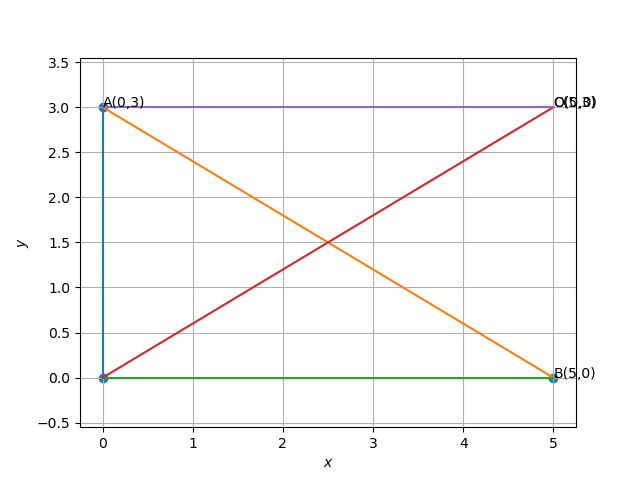
\includegraphics[width = 0.7\columnwidth]{figs/img.png}
    \caption*{}
    \label{figs}
\end{figure}

\end{document}